\subsection{Web application}
	La componente \textit{web app} ha il compito di interfacciare gli utenti con i dispositivi censiti dal sistema e visibili al loro ente di appartenenza.
	\newline
	Le principali funzionalità messe a disposizione riguardano la visualizzazione di grafici contenenti i dati di determinati sensori, la modifica delle configurazioni dei gateway e l'aggiunta o la rimozione di dispositivi e/o sensori.
	\newline 
	La componente è stata sviluppata utilizzando i framework Laravel e Vue.js.
	
	\subsubsection{Diagramma dei package}%%%%%%%%%OK
		\begin{figure}[H]
			\centering
			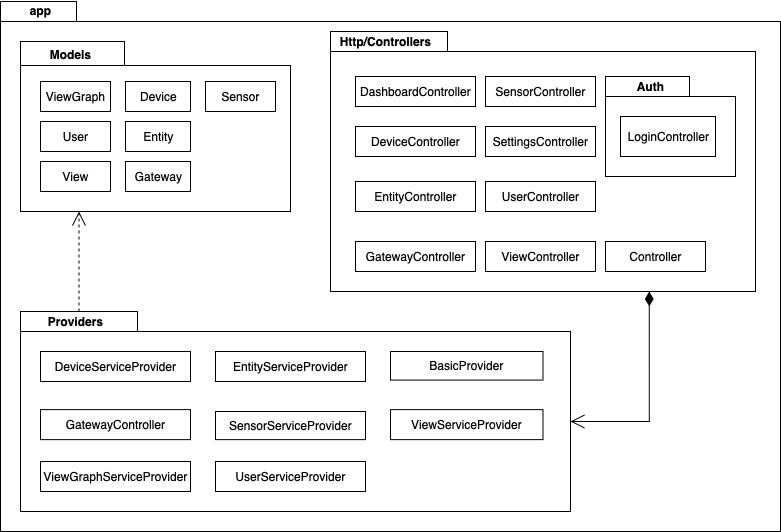
\includegraphics[scale=0.450]{res/images/WEBAPP/WebAppPackage.png}
			\caption{Diagramma dei package della componente web app}
			\label{Diagramma 21}
		\end{figure}
	
	\subsubsection{Dipendenze esterne}
		La componente ha le seguenti dipendenze esterne:
		\begin{itemize}
			\item \textbf{Laravel}, framework alla base della webapp, da cui vengono prese le basi dei controllers e dei models. Inoltre è il gestore delle view;
			\item \textbf{Laravel/UI}, viene utilizzata per l'autenticazione all'interno della webapp;
			\item \textbf{guzzlehttp/guzzle}, viene utilizzata per effettuare richieste HTTP in linguaggio PHP;
			\item \textbf{Axios}, viene utilizzata per effettuare delle richieste HTTP in Javascript;
			\item \textbf{Datatables.js}, viene utilizzata per la paginazione delle tabelle;
			\item \textbf{Apexcharts}, viene utilizzata per fare i grafici visibili all'interno dell'applicazione web;
			\item \textbf{davejamesmiller/laravel-breadcrumbs}, questa dipendenza viene utilizzata per generare i breadcrumb all'interno delle pagine visualizzate;
			\item \textbf{Vue.js}, framework che permette, tra le altre cose, di utilizzare array e variabili all'interno delle pagine per permetterne una visualizzazione dinamica dei contenuti;
			\item \textbf{Bootstrap}, framework utilizzato per la creazione dell'interfaccia grafica dell'applicazione web;
			\item \textbf{JQuery}, libreria utilizzata da Bootstrap per molte delle sue componenti;
			\item \textbf{Popper.js}, altra libreria utilizzata da Bootstrap.
		\end{itemize}


	\begin{landscape}
	\subsubsection{Diagrammi delle classi}%%%%%%%%%%OK
		\begin{figure}[H]
			\centering
			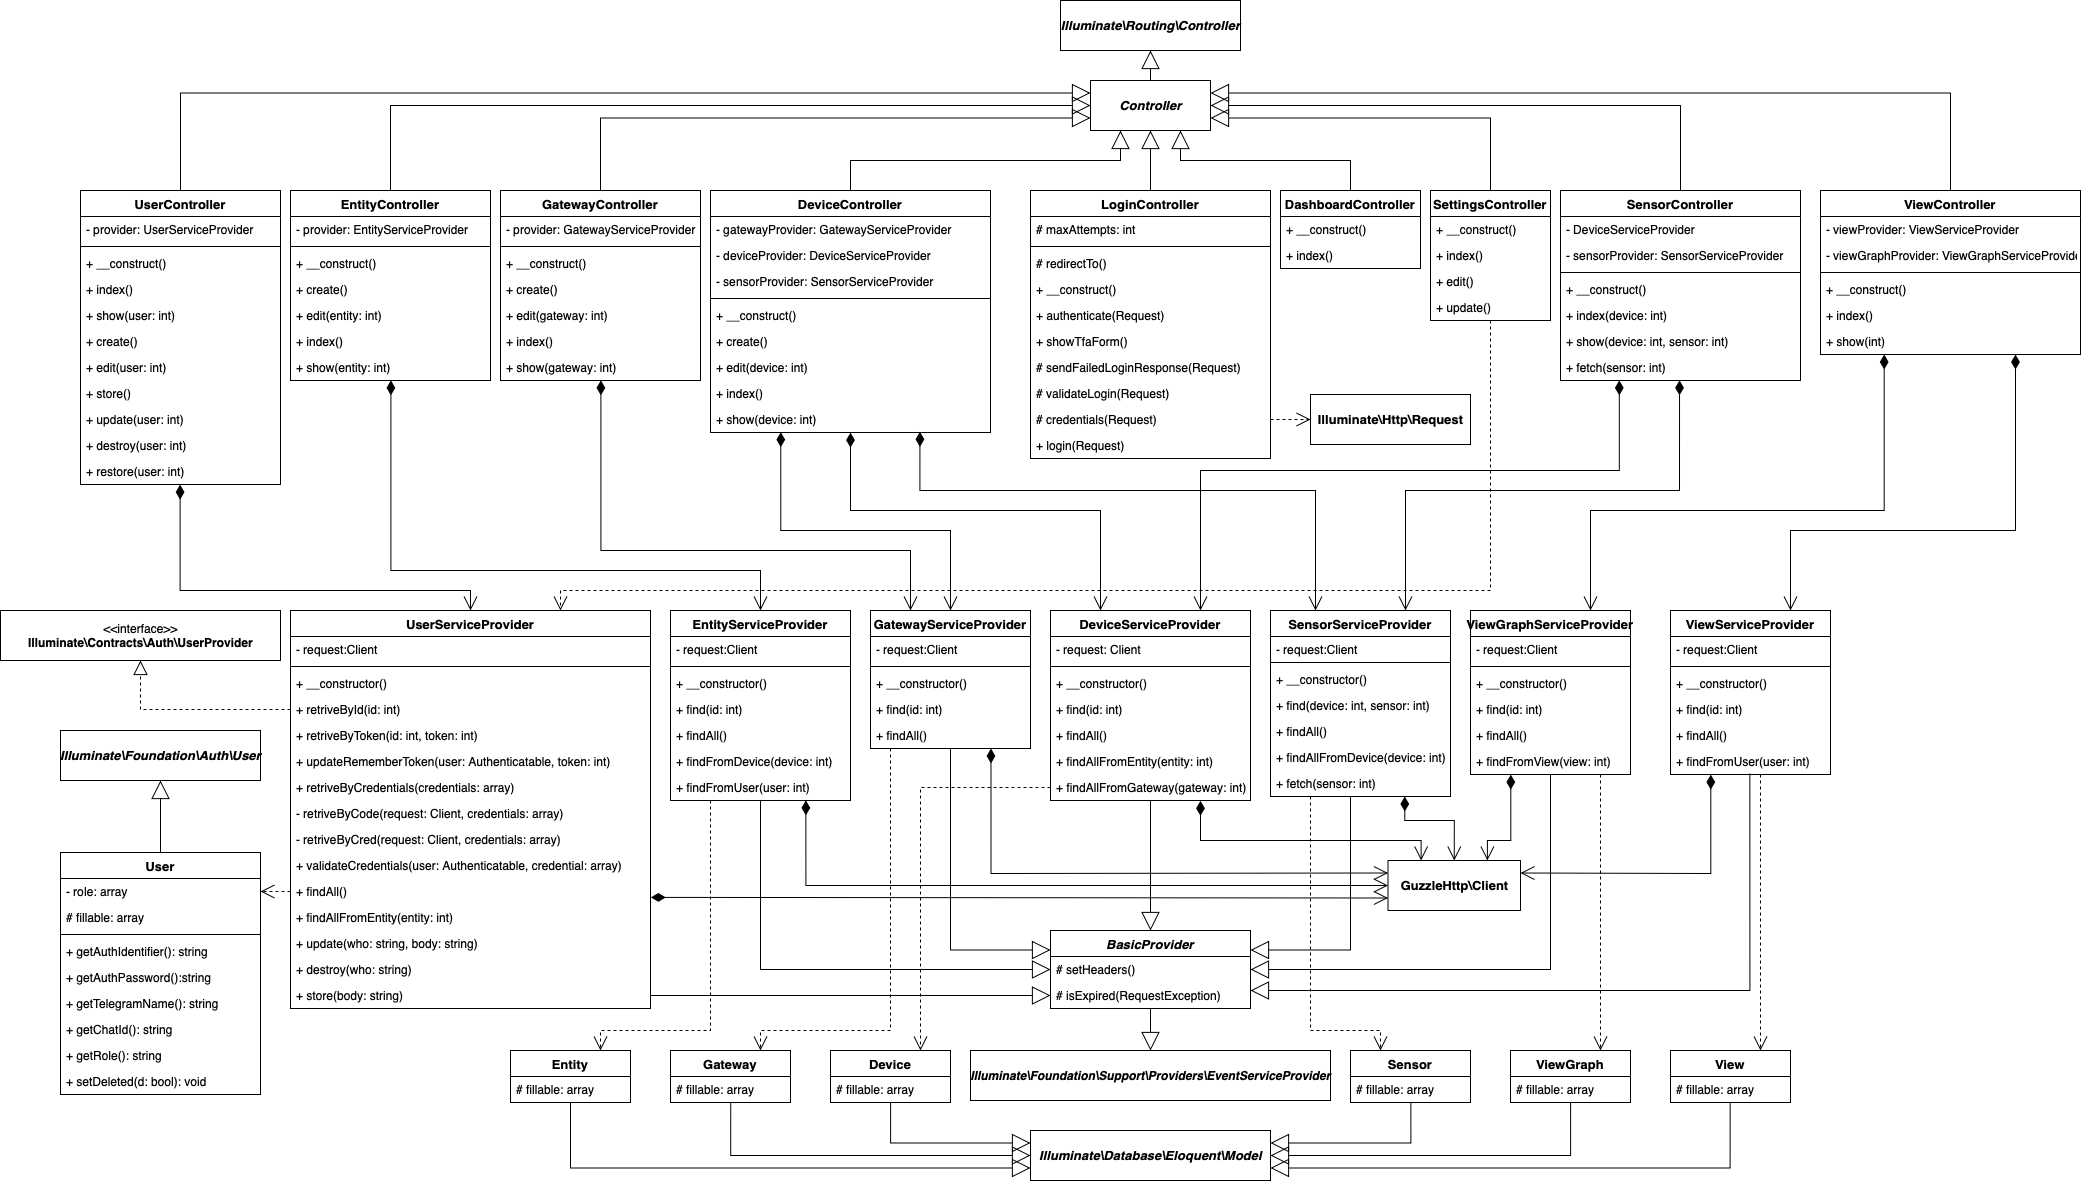
\includegraphics[scale=0.350]{res/images/WEBAPP/ClassiWebApp.png}
			\caption{Diagramma delle classi della componente web app}
			\label{Diagramma 22}
		\end{figure}
	\subsubsection{Diagrammi di sequenza}%%%%%%%%%%OK
		\begin{figure}[H]
			\centering
			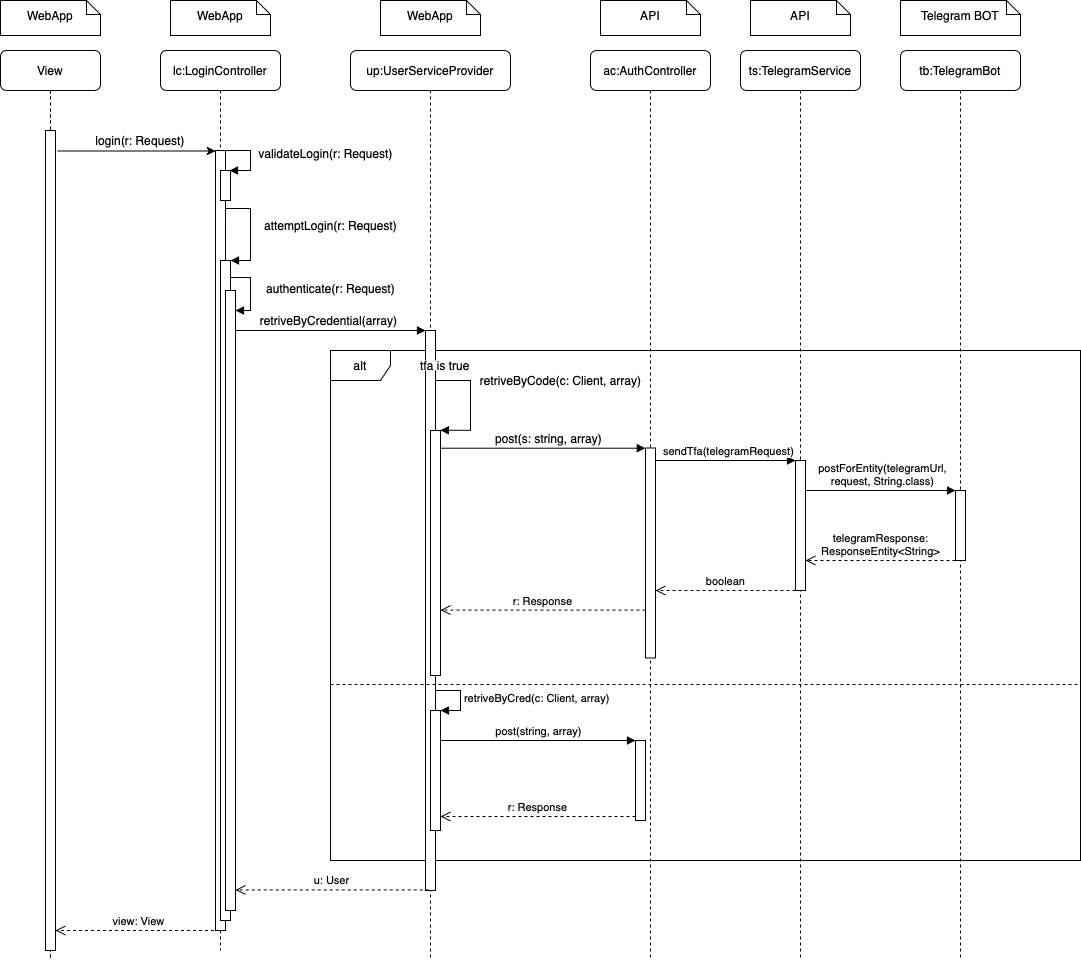
\includegraphics[scale=0.425]{res/images/WEBAPP/AutenticazioneTfa.png}
			\caption{Diagramma di sequenza che illustra l'autenticazione a due fattori all'interno della componente web app}
			\label{Diagramma 23}
		\end{figure}
		\begin{figure}[H]
			\centering
			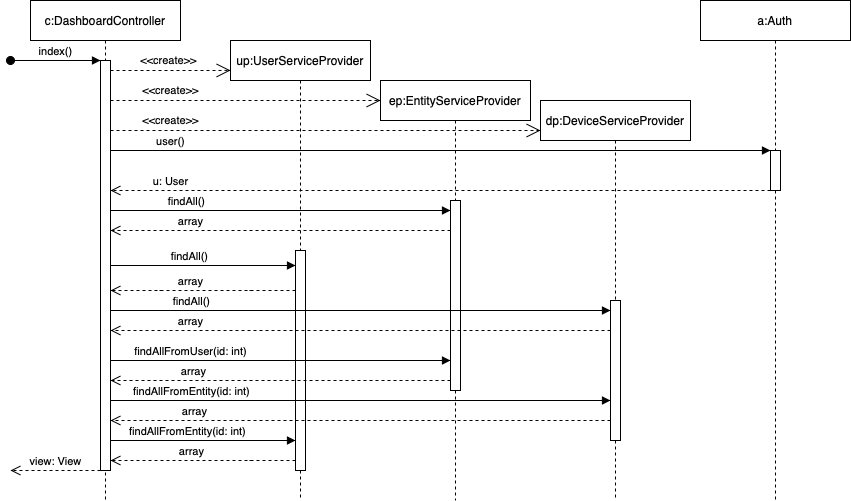
\includegraphics[scale=0.600]{res/images/WEBAPP/Dashboard.index.png}
			\caption{Diagramma di sequenza che illustra la visualizzazione della schermata dashboard all'interno della componente web app}
			\label{Diagramma 24}
		\end{figure}
	\end{landscape}